
\chapter{Storage Classes}
\label{chap:Storage}
This section details the different storage classes available in the system. The storage classes are designed to give efficient and fast storage in the system. The definitions are given below.
\section {Global variables and Data structures to store data }
\label{sec:Global Variables and structure data types}  
\subsection{ Storage Container for the Images}
\label{subsubsec:Datatypes} 
OpenCV defines Mat [Section \ref{sec:OpenCV}] as the default storage container for images. This custom storage container consists of a variable of type Mat, which is an OpenCV defined storage class for images. The container also consists of a variable defining the total number of points detected in the image.
\paragraph{Synopsis:}
\begin{lstlisting}
struct ImageMat{
       Mat img;
       int number_points_detected;
       ImageMat(){
        number_points_detected=0;
       }
};
\end{lstlisting}
\pagebreak
\paragraph{Example:} The method to define an object of the above defined structure is given below.
\begin{lstlisting}
main(){
    .
    .
    .
    ImageMat I;
    .
    .
    .
 }
\end{lstlisting}
\subsection{Storage Container for Point}
The storage of a point consists of a structure named coordinate and a \textit{structure} named \textit{RGB}. The structure consists of a variable of type \textit{time\_t}. The variable \textit{time\_t} defines current time at which a point is detected in the image. To track the points between corresponding frames and the successive images, a \textit{label} is introduced. Figure \ref{fig:structure definition point} shows the storage structure.
\paragraph{Synopsis:}
\begin{lstlisting}
struct point{
    string   label;
    time_t      t; 
    coordinates P;
    RGB         C;
};
\end{lstlisting}
\pagebreak
\paragraph{Example:}
The method to define an object of the above-defined structure is given below.
\begin{lstlisting}
main(){ 
    .
    .
    .
    point P;
    .
    .
    .
}    
\end{lstlisting}
\begin{figure}[ht]
    \centering
    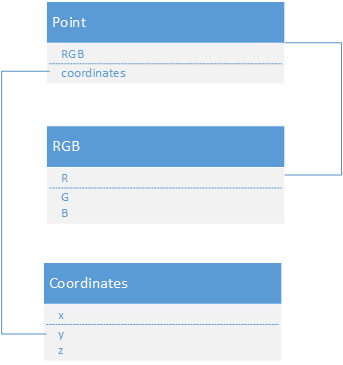
\includegraphics[width=10cm,height=10cm,keepaspectratio]{Pictures/point}
    \caption{Structure point definition}
    \label{fig:structure definition point}
\end{figure}
\subsection{Storage Container for Color}
 This container consists of three variables named \textit{R, G and B }corresponding to the three color parts of an image. Each of these has a range from 0-255, corresponding to each channel in the image as shown in Figure \ref{fig:RGB}.
\paragraph{Synopsis:}
\begin{lstlisting}
struct RGB{
        int R;
        int G;
        int B;
    RGB (){
        R=0;
        G=0;
        B=0;
    }
};
\end{lstlisting}
\paragraph{Example:}
The method to define an object of the above-defined structure is given below.
\begin{lstlisting}
main(){ 
    .
    .
    .
    RGB R;
    .
    .
\end{lstlisting}
\pagebreak
\begin{lstlisting}
    .
}  
\end{lstlisting}
\begin{figure}[ht]
    \centering
    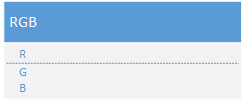
\includegraphics[width=12cm,height=12cm,keepaspectratio]{Pictures/RGB}
    \caption{Color}
    \label{fig:RGB}
\end{figure}
\subsection{Storage Container for Coordinates}
This data structure defines three variables \textit{x, y and z} which are the three coordinate values of a point in space. This can be used as a vector to store coordinates of any point in space. These variables are declared as float, so they can record different types of values as shown in Figure \ref{fig:XYZ}.
\paragraph{Synopsis:}
\begin{lstlisting}
struct coordinates{
    float x;
    float y;
    float z;
    coordinates(){
        x=0.0;
        y=0.0;
        z=0.0;
    };
\end{lstlisting}
\paragraph{Example:}
The method to declare a structure is given below.
\begin{lstlisting}
main(){ 
    .
    .
    .
    coordinates R;
    .
    .
    .
} 
\end{lstlisting}
\begin{figure}[ht]
    \centering
    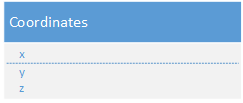
\includegraphics[width=8cm,height=8cm,keepaspectratio]{Pictures/Coordinatesxyz}
    \caption{Coordinates}
    \label{fig:XYZ}
\end{figure}
\subsection{Storage Container for Lines}
A structure containing an object of type points is used to store lines, consists of two variables, one that stores the vertices of the line and the other one points to the next vertex in the image. In a chain of points , if a point is found, that is same as the starting point then it describes a closed polygon otherwise a piecewise straight line. 
\pagebreak
\paragraph{Synopsis:}
\begin{lstlisting}
struct lines{
    point vertex;
    lines *next;
};
\end{lstlisting}
\paragraph{Example:}
The method to declare a structure is given below.
\begin{lstlisting}
main(){ 
    .
    .
    .
    lines *L=new lines();
    .
    .
    .
}
\end{lstlisting}
\section{Permanent Storage}
 Permanent storage of data is very important, and the  retrieval and storage should take minimum time. For this purpose four structures are defined as part of the system. There are structures respectively for storing images; point; lines and motion. All the four structures can be accessed using a key, which is defined by the user. All the keys, that are used for storage, are also stored in a variable array, and the user can read, edit and remove the keys anytime using the functions provided in the library. The usage and definition of these structures and functions are given below.
\subsection{Maps/Associative Array Structure to Store an Image}
This structure consists of three variables, one is an associative array for the storage of image, and the other two variables are the storage for keys, which are used to store data. The primary key is a user specifiable string. The second or the inner key is time. An image may be stored at different times, giving the user the ability to track the behavior of an image at different times as shown in Figure \ref{fig:map}. 
\paragraph{Synopsis:}
\begin{lstlisting}
struct I_List{
map < pair<string, time_t>, ImageMat> Images_List;
std::vector<std::string>   keyouterImages;
vector<time_t>   keytimeImages;   
};
\end{lstlisting}
\subsection{Maps/Associative Array Structure  to Store Points}
    The permanent storage of points is done in this associative array. The primary key is a string that is specified by the user, this string can also be the label of a point in the image. The second or the inner key is time. A certain kind of point may be stored at different times, giving the ability to track the behavior of the point at different times as shown in Figure \ref{fig:map}.
\paragraph{Synopsis:}
\begin{lstlisting}
struct P_List{
map < pair<string, time_t>, point   > Points_List;
vector<string>   keyouterPoints;
\end{lstlisting}
\pagebreak
\begin{lstlisting}
vector<time_t>   keytimePoints;  
};
\end{lstlisting}
\subsection{Maps/Associative Array Structure to Store Lines}
     A structure similar to the one presented in Section 4.2.2. is used to store lines. An associative array to store the lines and two other arrays to store the keys is also provided in the system as shown in Figure \ref{fig:map}.
\paragraph{Synopsis:}
\begin{lstlisting}
struct L_List{
map < pair<string, time_t>, lines*   > Lines_List;
vector<string>   keyouterLines;
vector<time_t>   keytimeLines;  
};
\end{lstlisting}

\subsection{Maps/Associative Array Structure to Store Camera Motion}
    The permanent storage of camera motion is done in this associative array. The primary key is the time. The structure is similar to the one in section 4.2.2. It has one other variable to store the key as shown in Figure \ref{fig:map}.

\paragraph{Synopsis:}
\begin{lstlisting}
struct M_Lidst{
map < time_t, Matx34d > TrackMotion; 
vector<time_t>   keytimemotion;  
}; 
\end{lstlisting}
There are functions provided in the library, that can be used for storing data using the associative array and also can be used for editing and removing the keys from the array. The description about these functions is given in Low Level function Section. Figure \ref{fig:map} explains the storage of data in an associative array.
\begin{figure}[ht]
    \centering
    \includegraphics[width=15cm,height=15cm,keepaspectratio]{Pictures/map.png}
    \caption{Map Memory Storage}
    \label{fig:map}
\end{figure}

\subsection{Maps/Associative Array Structure to Store Coordinates\_List}
This list is to keep track of all the points that are detected in the images. Whenever a point is labeled or found, they are stored in this array. When a point is detected, it is compared with the points in this list and if a close proximity is established, then the points in the proximity are labeled the same.
\paragraph{Synopsis:}
\begin{lstlisting}
std::vector<point> coordinates_list;
\end{lstlisting}
\begin{figure}[ht]
    \centering
    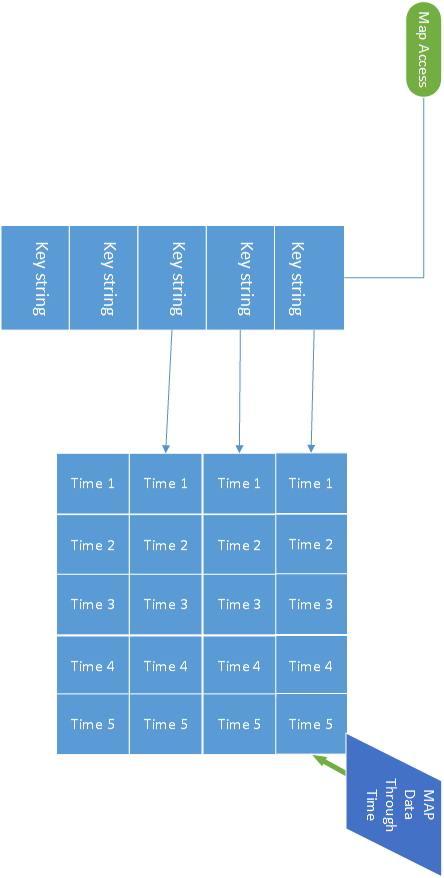
\includegraphics[width=20cm,height=20cm,keepaspectratio]{Pictures/map_1.png}
    \caption{Associate Memory Access}
    \label{fig:map1}
\end{figure}

\subsection{Maps/Associative Array Structure to Store TrackMotion}
This list keeps track of all the motion. The camera motion matrix, that is the transformation between, the two positions of the camera, is stored in this array. 

The first entry in this matrix is the initial projection matrix, that is the transformation between the image plane and the real world plane. This matrix is tracked with respect to time.
\paragraph{Synopsis:}
\begin{lstlisting}
map < time_t,  Matx34d > TrackMotion; 
\end{lstlisting}

